\begin{appendix}

\eat{
% clustering
\begin{figure*}[b]
    \centering
    \begin{minipage}[b]{0.32\linewidth}
        \centering
        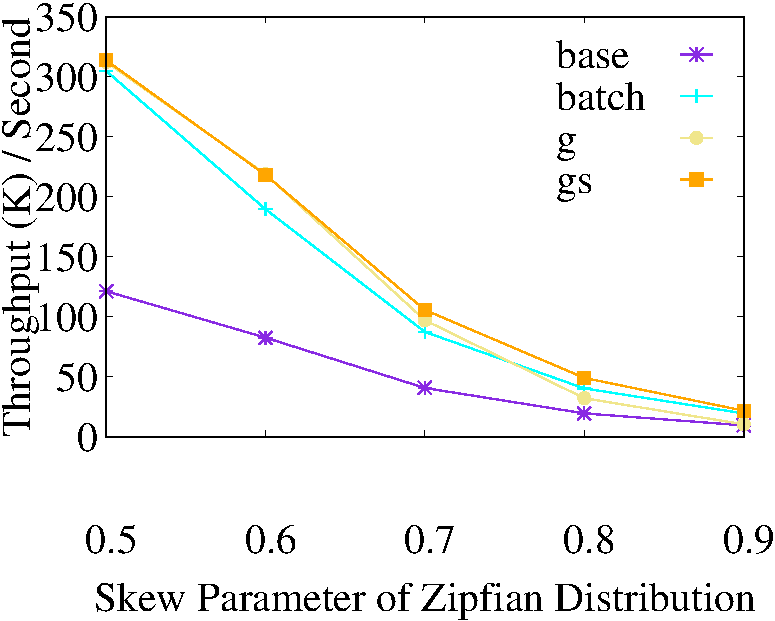
\includegraphics[width=\textwidth]{./exp_fig/cluster/tps}
        \vspace{-2em}
        \caption{Throughput with validator clustering}
        \label{fig:cluster:tps}
    \end{minipage}
    \begin{minipage}[b]{0.32\linewidth}
        \centering
        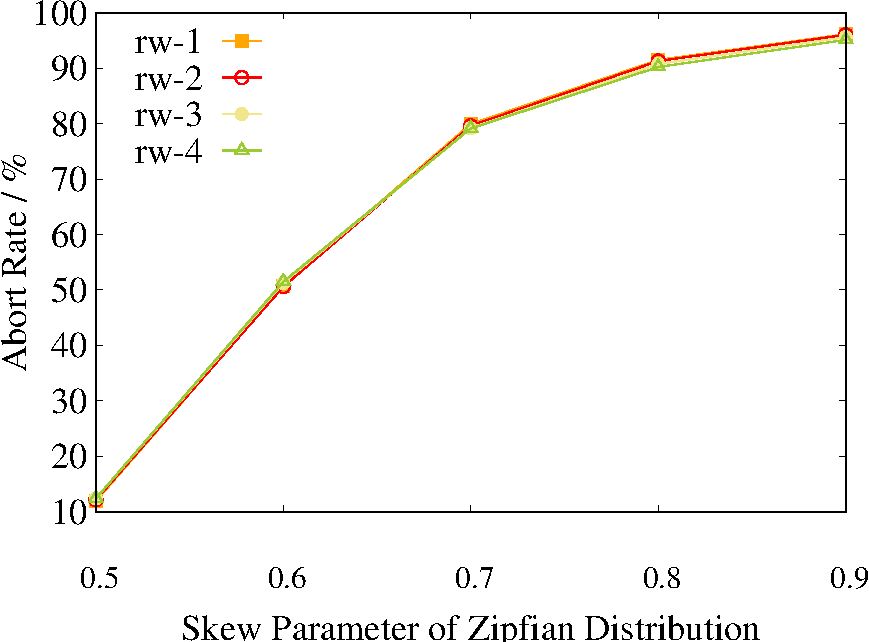
\includegraphics[width=\textwidth]{./exp_fig/cluster/abort}
        \vspace{-2em}
        \caption{Abort rate with validator clustering}
        \label{fig:cluster:abort}
    \end{minipage}
    \begin{minipage}[b]{0.32\linewidth}
        \centering
        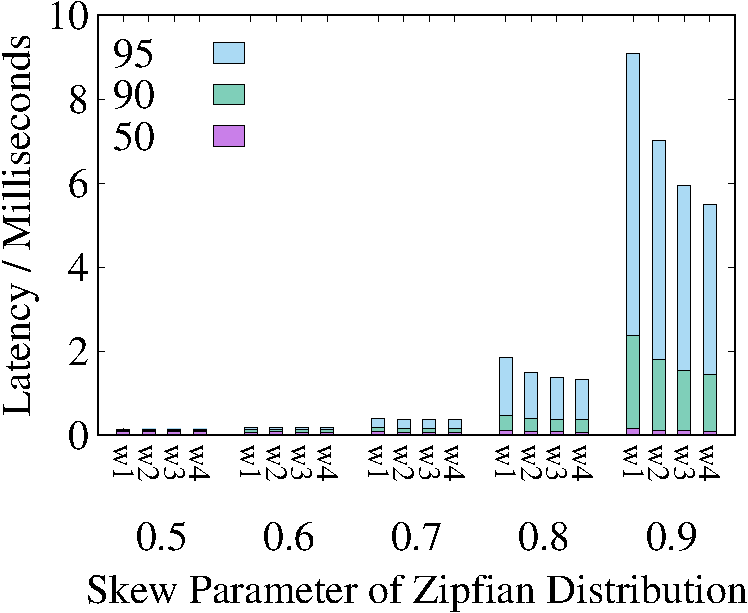
\includegraphics[width=\textwidth]{./exp_fig/cluster/percent95_latency}
        \vspace{-2em}
        \caption{Percentile latency with validator clustering}
        \label{fig:cluster:p95}
    \end{minipage}
\end{figure*}
}

% end to end experiment: load
\begin{figure*}[b]
    \centering
    \begin{minipage}[b]{0.32\linewidth}
        \centering
        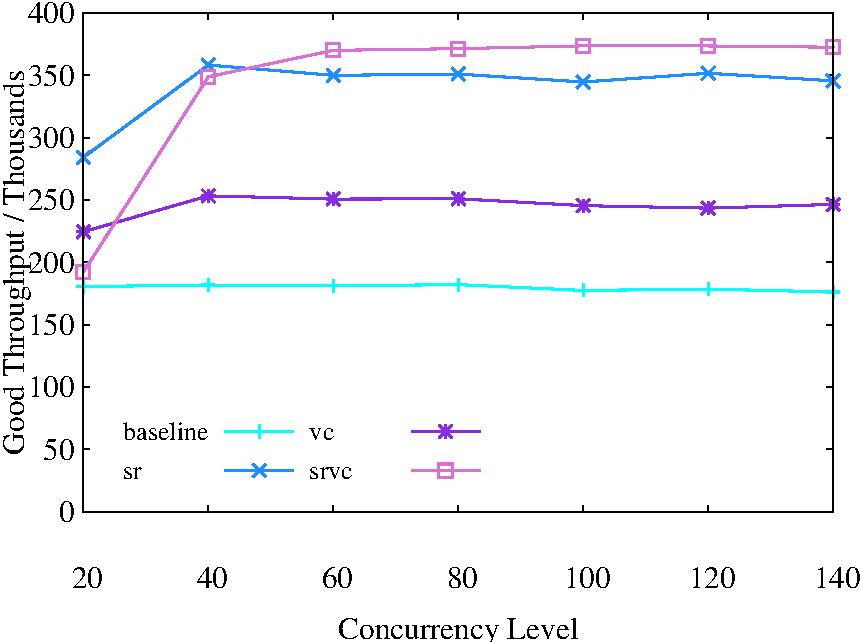
\includegraphics[width=\textwidth]{{{./exp_fig/load/Z0.5.tps}}}
        \vspace{-2em}
        \caption{Throughput when varying the load (skew factor: 0.5)}
        \label{fig:load:z0.5:tps}
    \end{minipage}
    \begin{minipage}[b]{0.32\linewidth}
      	\centering
        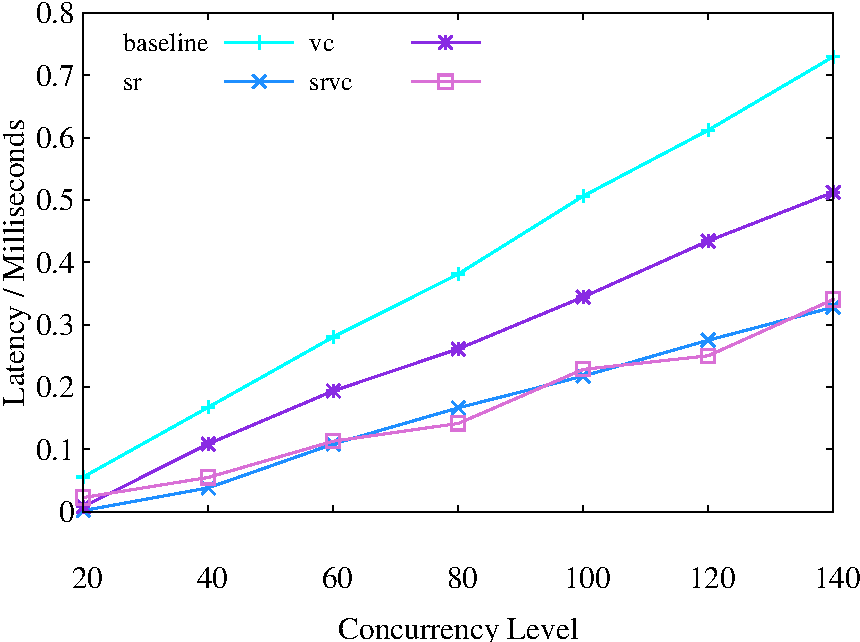
\includegraphics[width=\textwidth]{{{./exp_fig/load/Z0.5.latency}}}
        \vspace{-2em}
        \caption{Average latency when varying the load (skew factor: 0.5)}
        \label{fig:load:z0.5:latency}
    \end{minipage}
    \begin{minipage}[b]{0.32\linewidth}
        \centering
        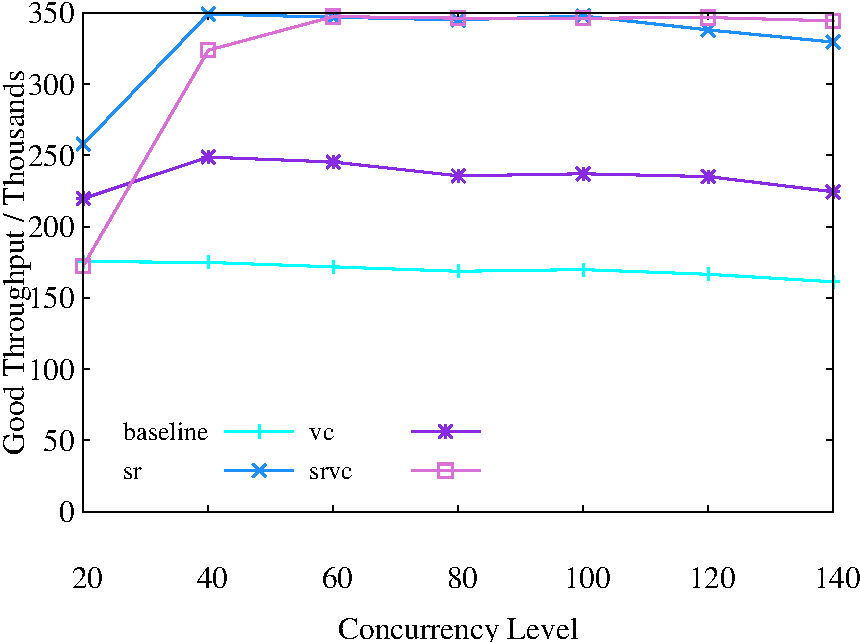
\includegraphics[width=\textwidth]{{{./exp_fig/load/Z0.6.tps}}}
        \vspace{-2em}
        \caption{Throughput when varying the load (skew factor: 0.6)}
        \label{fig:load:z0.6:tps}
    \end{minipage}
\end{figure*}    
   
\begin{figure*}[b]
	\centering
    \begin{minipage}[b]{0.32\linewidth}
      	\centering
        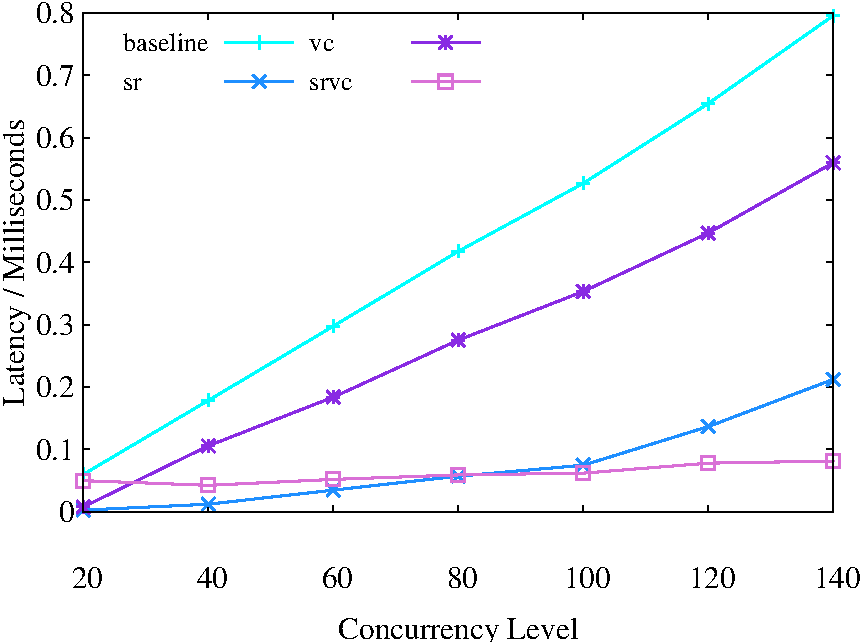
\includegraphics[width=\textwidth]{{{./exp_fig/load/Z0.6.latency}}}
        \vspace{-2em}
        \caption{Average latency when varying the load (skew factor: 0.6)}
        \label{fig:load:z0.6:latency}
    \end{minipage}
    \begin{minipage}[b]{0.32\linewidth}
        \centering
        \includegraphics[width=\textwidth]{{{./exp_fig/load/Z0.8.tps}}}
        \vspace{-2em}
        \caption{Throughput when varying the load (skew factor: 0.8)}
        \label{fig:load:z0.8:tps}
    \end{minipage}
    \begin{minipage}[b]{0.32\linewidth}
      	\centering
        \includegraphics[width=\textwidth]{{{./exp_fig/load/Z0.8.latency}}}
        \vspace{-2em}
        \caption{Average latency when varying the load (skew factor: 0.8)}
        \label{fig:load:z0.8:latency}
    \end{minipage}
\end{figure*}

\begin{figure*}[b]
    \centering
    \begin{minipage}[b]{0.32\linewidth}
        \centering
        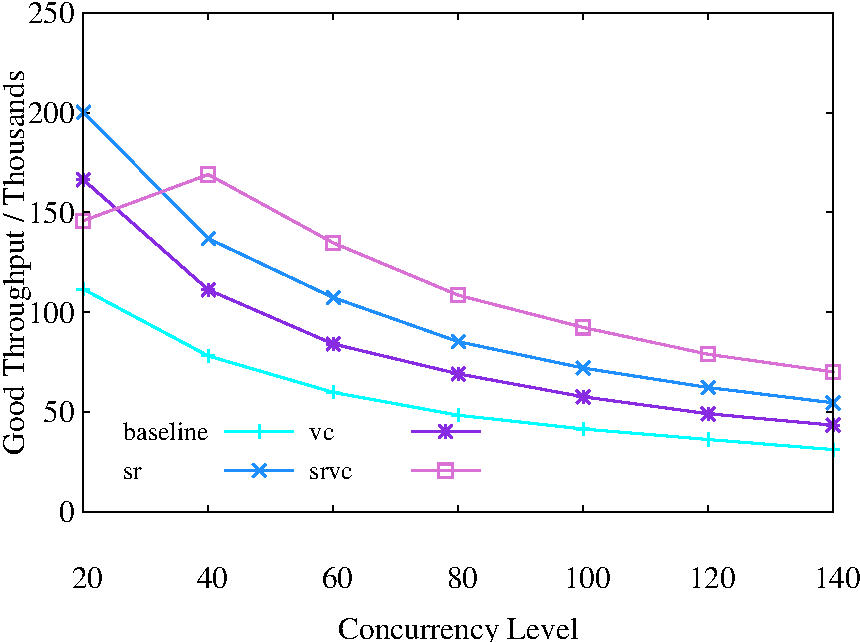
\includegraphics[width=\textwidth]{{{./exp_fig/load/Z0.9.tps}}}
        \vspace{-2em}
        \caption{Throughput when varying the load (skew factor: 0.9)}
        \label{fig:load:z0.9:tps}
    \end{minipage}
    \begin{minipage}[b]{0.32\linewidth}
      	\centering
        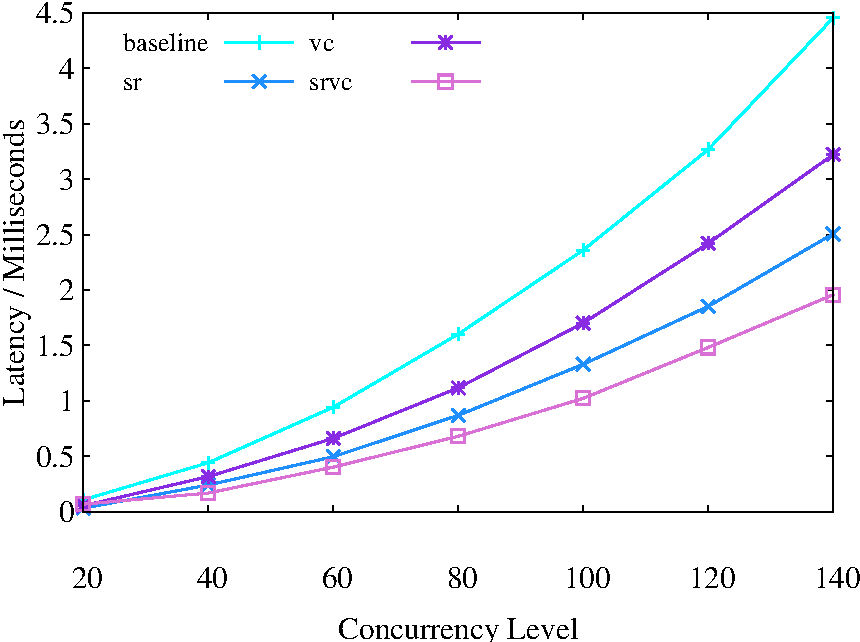
\includegraphics[width=\textwidth]{{{./exp_fig/load/Z0.9.latency}}}
        \vspace{-2em}
        \caption{Average latency when varying the load (skew factor: 0.9)}
        \label{fig:load:z0.9:latency}
    \end{minipage}
    \begin{minipage}[b]{0.32\linewidth}
        \centering
        \includegraphics[width=\textwidth]{{{./exp_fig/small_bank/Z0.8.tps}}}
        \vspace{-2em}
        \caption{Throughput with Small Bank benchmark (skew factor: 0.8)}
        \label{fig:small_bank:z0.8:tps}
    \end{minipage}
\end{figure*}

\begin{figure*}[htbp]
    \centering
    \begin{minipage}[b]{0.32\linewidth}
        \centering
        \includegraphics[width=\textwidth]{{{./exp_fig/small_bank/Z0.8.latency}}}
        \vspace{-2em}
        \caption{Average latency with Small Bank benchmark (skew factor: 0.8)}
        \label{fig:small_bank:z0.8:latency}
    \end{minipage}
\end{figure*}

\eat{
\section{Validator Reordering Policies}
\label{subsec:appendix:policy}
In this section, we show additional policies on validator reordering for heterogeneous workloads, including prioritizing hard transactions and validator clustering.
\subsection{Validator Clustering}
In this experiment, we explore the performance impact of clustering by access patterns for validator batch creation as described in Section~\ref{subsec:overview:validator}. Since we do not introduce new clustering techniques in the paper, we hardcode a ``clustering'' strategy by partitioning the data into 2 equal partitions beforehand, and generating transactions based on the data partitions. Each transaction randomly chooses a partition as its home data partition. For each item it accesses, there is a 90\% chance that the item is from its home partition, and a 10\% chance that the item is from the other remote data partition. The transaction follows a Zipfian distribution when choosing items within a data partition.

We compare the system performance with validator clustering ($srvc\hbox{-}c$) and without validator clustering ($srvc$) when both storage and validator batching are enabled, as well as the baseline ($baseline$). Figure~\ref{fig:cluster:tps} shows the system throughput. Validator clustering can reduce throughput due to higher latencies, especially when the skew is high. On the other hand, as shown in Figure~\ref{fig:cluster:abort} and Figure~\ref{fig:cluster:p95}, it gives a much better abort rate and percentile latency, since it reduces both inter- and intra-batch conflicts. 
}

\section{End-to-End Performance}
\label{subsec:appendix:end2end}

This section shows additional end-to-end experiment results on micro benchmark and Small Bank benchmark.

For our micro benchmark, we run the system under additional skew factors: 0.5 (Figure~\ref{fig:load:z0.5:tps} and Figure~\ref{fig:load:z0.5:latency}), 0.6 (Figure~\ref{fig:load:z0.6:tps} and Figure~\ref{fig:load:z0.6:latency}), 0.8 (Figure~\ref{fig:load:z0.8:tps} and Figure~\ref{fig:load:z0.8:latency}), and 0.9 (Figure~\ref{fig:load:z0.9:tps} and Figure~\ref{fig:load:z0.9:latency}). Comparing to the baseline, the results are similar as what we observe in Section~\ref{subsec:experiment:end2end}: batching always largely increases the throughput for both fixed load and the peak throughput over various loads; it also halves the average latency. While adding validator batching always outperforms storage batching alone when the load is demanding, sometimes storage batching alone achieves the peak throughput over various loads. 

Figure~\ref{fig:small_bank:z0.8:tps} and Figure~\ref{fig:small_bank:z0.8:latency} shows the throughput and the latency of Small Bank benchmark with skew factor 0.8. The overall performance characteristic is similar to the results in Section~\ref{subsec:experiment:end2end}.

\end{appendix}
